\chapter{Diagrama de estados}

\par Este documento recoge el diagrama de transición de estados de la clase Sensor de punto ciego.

\begin{figure}[h]
\begin{center}
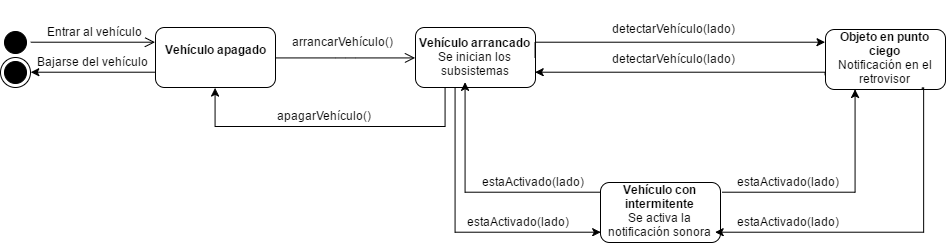
\includegraphics[width=1\textwidth]{./img/diagramadeestados.png}
\end{center}
\caption{Diagrama de estados de la clase Sensor de punto ciego.}
\label{tab:d_EstadosPNG}
\end{figure}

\par En un primer momento, el sistema se encuentra apagado, ya que el vehículo se encuentra apagado. Por lo tanto,
se necesitará que el usuario se suba al vehículo. A partir de ese hecho, se pueden identificar cuatro estados:
\begin{itemize}
  \item \textbf{Vehículo apagado}: Es el estado inicial. En este estado ninguno de los subsistemas está iniciado.
  \item \textbf{Vehículo arrancado}: Cuando el vehículo se pone en marcha, también se inicial los subsistemas.
  \item \textbf{Objeto en punto ciego}: Si el sensor detecta un objeto en el punto ciego, pasa a este estado, donde genera una notificación en el retrovisor.
  \item \textbf{Vehículo con intermitente}: Cuando el conductor activa un intermitente y hay un objeto en el punto ciego, se genera una notificación sonora.
\end{itemize}

\par Cuando se encuentra en el estado Vehículo apagado, solo puede pasar al estado Vehículo arrancado mediante el método arrancarVehículo(). Asimísmo, solo se puede llegar a
este estado desde Vehículo arrancado con el método apagarVehículo().

Desde vehículo arrancado se puede llegar a Objeto en punto ciego, si el método detectarVehículo() detecta un vehículo en el punto ciego. Desde esta clase se puede volver al estado
vehículo arrancado si dicho método no detecta un objeto en el punto ciego.

Por último, desde Objeto en punto ciego y Vehículo arrancado se puede llegar a Vehículo con intermitente si se detecta que el conductor ha activado un intermitente.
